\documentclass[11pt,a4paper]{article}
\usepackage[utf8]{inputenc}
\usepackage[T1]{fontenc}
\usepackage{lmodern}
\usepackage[margin=1.8cm,top=1.8cm,bottom=1.8cm]{geometry}
\usepackage{amsmath,amssymb}
\usepackage{booktabs}
\usepackage{tabularx}
\usepackage{array}
\usepackage{enumitem}
\usepackage{float}
\usepackage[table]{xcolor}
\usepackage{colortbl}
\usepackage{tikz}
\usetikzlibrary{shapes.geometric,arrows.meta,positioning,fit,calc,backgrounds}
\usepackage{fancyhdr}
\usepackage{titlesec}
\usepackage{microtype}
\usepackage[colorlinks=true,linkcolor=blue!70!black,citecolor=blue!70!black,urlcolor=blue!70!black]{hyperref}

% Header and Footer styling
\pagestyle{fancy}
\fancyhf{}
\fancyhead[L]{\small\textsf{\textbf{Part 3: The Guardian} \textbar\ 3-Layer Urban IoT Monitoring Platform}}
\fancyhead[R]{\small\textsf{Page \thepage}}
\fancyfoot[L]{\small\textsf{Guardian Layer Team Report \textbar\ Version 1.0}}
\fancyfoot[R]{\small\textsf{NIST SP 800-207 / 800-57 / ISO 27001}}
\renewcommand{\headrulewidth}{0.5pt}
\renewcommand{\footrulewidth}{0.5pt}

% Section formatting
\titleformat{\section}
  {\normalfont\sffamily\Large\bfseries\color{blue!80!black}}
  {\thesection}{0.8em}{}
\titleformat{\subsection}
  {\normalfont\sffamily\large\bfseries\color{blue!70!black}}
  {\thesubsection}{0.6em}{}
\titleformat{\subsubsection}
  {\normalfont\sffamily\normalsize\bfseries\color{black}}
  {\thesubsubsection}{0.5em}{}

\titlespacing*{\section}{0pt}{6pt}{3pt}
\titlespacing*{\subsection}{0pt}{5pt}{2pt}
\titlespacing*{\subsubsection}{0pt}{3pt}{1pt}
\setlength{\parskip}{2pt}
\setlength{\parindent}{0pt}

\begin{document}

\setcounter{section}{2} % Starts section numbering at 3

\section{The Guardian}

\subsection{Role and goals}
Positioned between the Digital Twin (sensor simulation and ingestion) and the City Brain (supervisory control and actuation), the Guardian serves as the untrusted-input gatekeeper of the 3-layer urban monitoring architecture. Field telemetry from drainage networks and power grids is vulnerable to tampering, transmission noise, and hardware faults. The Guardian establishes an active defensive perimeter: it cryptographically verifies message origin, drops malformed payloads, buffers readings in sliding memory windows, extracts spatio-temporal features, and runs machine learning inference to classify anomalies before clean data reaches the Brain.

The Guardian is engineered against four measurable operational goals:
\begin{enumerate}[leftmargin=*,itemsep=1pt,topsep=2pt]
  \item \textbf{Real-time verification latency:} Short-window anomaly scoring under 150\,ms per window ($p_{50} = 102$\,ms, $p_{99} = 123$\,ms for 42 sensors $\times$ 200 readings), operating within the 10\,s streaming interval ($>98\%$ CPU margin).
  \item \textbf{Strict false alarm budget:} Under 0.04 false alarms per sensor-day on clean streams, measured empirically at 0.008 false alarms/sensor-day on the 24\,h model with 0.951 PR-AUC.
  \item \textbf{High-throughput edge buffering:} Buffer ingestion at 2.75\,$\mu$s per reading ($>360,000$ ops/s per core) with fail-safe rollback to prevent data loss during downstream queue saturation.
  \item \textbf{Cryptographic non-repudiation:} 100\% asymmetric Ed25519 signature verification on untrusted ingest streams prior to state admission.
\end{enumerate}

\noindent\textit{Scope boundaries:} In scope: signature verification, schema translation, sliding ring buffering, static rule checks, dual-horizon XGBoost anomaly scoring, and DLQ routing. Out of scope: sensor simulation (Twin), supervisory actuation (Brain), and enterprise data warehousing.

\subsection{Architecture}
The Guardian pipeline enforces a sequential defensive progression from signed ingestion to final verdict emission, as shown in Figure~\ref{fig:guardian_arch}.

\begin{figure}[H]
\centering
\resizebox{\textwidth}{!}{%
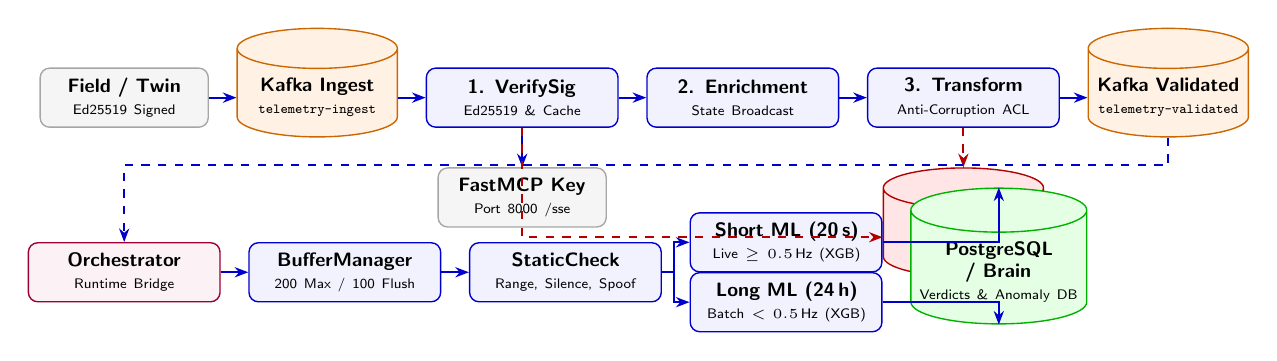
\begin{tikzpicture}[
    node distance=0.35cm and 0.4cm,
    font=\sffamily\scriptsize,
    box/.style={rectangle, draw=blue!80!black, fill=blue!5!white, rounded corners=1.2mm, minimum height=0.75cm, text width=2.2cm, align=center, line width=0.5pt},
    queue/.style={cylinder, shape border rotate=90, draw=orange!80!black, fill=orange!10!white, aspect=0.25, minimum height=0.75cm, text width=1.8cm, align=center, line width=0.5pt},
    extbox/.style={rectangle, draw=gray!70, fill=gray!8!white, rounded corners=1.2mm, minimum height=0.75cm, text width=1.9cm, align=center, line width=0.5pt},
    dlqbox/.style={cylinder, shape border rotate=90, draw=red!70!black, fill=red!10!white, aspect=0.25, minimum height=0.75cm, text width=1.8cm, align=center, line width=0.5pt},
    db/.style={cylinder, shape border rotate=90, draw=green!70!black, fill=green!10!white, aspect=0.25, minimum height=0.75cm, text width=2.0cm, align=center, line width=0.5pt},
    line/.style={-{Stealth[scale=0.8]}, draw=blue!80!black, line width=0.7pt},
    reject/.style={-{Stealth[scale=0.8]}, draw=red!70!black, dashed, line width=0.7pt}
]

% Row 1: Ingestion, Crypto Gate, Transformation
\node[extbox] (twin) {\textbf{Field / Twin}\\\tiny Ed25519 Signed};
\node[queue, right=0.35cm of twin] (raw) {\textbf{Kafka Ingest}\\\tiny \texttt{telemetry-ingest}};
\node[box, right=0.35cm of raw] (sig) {\textbf{1. VerifySig}\\\tiny Ed25519 \& Cache};
\node[box, right=0.35cm of sig] (enrich) {\textbf{2. Enrichment}\\\tiny State Broadcast};
\node[box, right=0.35cm of enrich] (trans) {\textbf{3. Transform}\\\tiny Anti-Corruption ACL};
\node[queue, right=0.35cm of trans] (val) {\textbf{Kafka Validated}\\\tiny \texttt{telemetry-validated}};

% Side services for Row 1
\node[extbox, below=0.5cm of sig] (mcp) {\textbf{FastMCP Key}\\\tiny Port 8000 /sse};
\node[dlqbox, below=0.5cm of trans] (dlq) {\textbf{Kafka DLQ}\\\tiny \texttt{telemetry-dlq}};

% Row 2: Buffering, Rules, ML Inference
\node[box, below=1.45cm of twin, fill=purple!5!white, draw=purple!80!black] (orch) {\textbf{Orchestrator}\\\tiny Runtime Bridge};
\node[box, right=0.35cm of orch] (buf) {\textbf{BufferManager}\\\tiny 200 Max / 100 Flush};
\node[box, right=0.35cm of buf] (static) {\textbf{StaticCheck}\\\tiny Range, Silence, Spoof};
\node[box, right=0.35cm of static, yshift=0.38cm] (short_pipe) {\textbf{Short ML (20\,s)}\\\tiny Live $\ge 0.5$\,Hz (XGB)};
\node[box, right=0.35cm of static, yshift=-0.38cm] (long_pipe) {\textbf{Long ML (24\,h)}\\\tiny Batch $< 0.5$\,Hz (XGB)};
\node[db, right=0.35cm of short_pipe, yshift=-0.38cm] (pg) {\textbf{PostgreSQL / Brain}\\\tiny Verdicts \& Anomaly DB};

% Connections Row 1
\draw[line] (twin) -- (raw);
\draw[line] (raw) -- (sig);
\draw[line] (sig) -- (enrich);
\draw[line] (enrich) -- (trans);
\draw[line] (trans) -- (val);
\draw[line] (sig) -- (mcp);
\draw[reject] (sig.south) |- (dlq.west);
\draw[reject] (trans) -- (dlq);

% Inter-row connection
\draw[line, dashed] (val.south) -- ++(0,-0.35) -| (orch.north);

% Connections Row 2
\draw[line] (orch) -- (buf);
\draw[line] (buf) -- (static);
\draw[line] (static.east) -- ++(0.15,0) |- (short_pipe.west);
\draw[line] (static.east) -- ++(0.15,0) |- (long_pipe.west);
\draw[line] (short_pipe.east) -| (pg.north);
\draw[line] (long_pipe.east) -| (pg.south);

\end{tikzpicture}
}
\caption{The Guardian Pipeline Architecture: Ingestion, Filtering, Buffering, and Dual-Horizon ML}
\label{fig:guardian_arch}
\end{figure}

The detection and filtering mechanisms operate across three sequential stages:
\begin{enumerate}[leftmargin=*,itemsep=2pt,topsep=2pt]
  \item \textbf{Cryptographic and schema gate (Stage 1):} Ingests raw JSON from \texttt{telemetry-ingest}, strips Base64 signature \texttt{sig}, and validates the Ed25519 signature over canonical compact JSON against FastMCP public keys. Catches forged payloads, unknown devices, syntax errors, and schema violations, routing rejects to \texttt{telemetry-dlq} with structured error codes (\texttt{E100}--\texttt{E320}) while dropping isolated/quarantined devices.
  \item \textbf{Static rule checks (Stage 2):} Deterministic sub-microsecond pre-filtering applied to flushed batches prior to ML inference. Catches out-of-range sensor values ($x < x_{\min} \lor x > x_{\max}$), silent dropouts (deltas $> 10.0$\,s), future-skewed timestamps, and gross spatial spoofing relative to cluster peers.
  \item \textbf{Machine learning detection (Stage 3):} Routes telemetry by sampling frequency across dual analytical horizons:
  \begin{itemize}[leftmargin=*,itemsep=1pt]
    \item \textit{Short-window model (20\,s live horizon, $\ge 0.5$\,Hz):} Evaluates Robust $Z$-scores (MAD scaling), Haar wavelets, difference kurtosis, sign-flip counts, and $k$-NN Haversine peer distances. Catches sudden spikes, oscillations, stuck values, burst noise, and synthetic signals (sine, ramp, pattern, uniform).
    \item \textit{Long-window model (24\,h batch horizon, $< 0.5$\,Hz):} Resamples telemetry onto a 300\,s time-grid, computing trend-to-scatter ratios, flatline runs, and cluster slope divergence. Catches slow multi-hour calibration drift and frozen monitors while distinguishing sensor degradation from regional weather shifts.
  \end{itemize}
\end{enumerate}

\subsection{Tech stack and why}
The Guardian tech stack balances sub-microsecond latency, type safety, zero-trust isolation, and empirical accuracy:

\begin{table}[H]
\centering
\scriptsize
\caption{Guardian Technology Stack and Empirical Selection Justification}
\label{tab:tech_stack}
\begin{tabularx}{\textwidth}{llX}
\toprule
\textbf{Component} & \textbf{Technology \& Version} & \textbf{Why Chosen (Empirical Justification \& Benchmarks)} \\
\midrule
\textbf{Language Runtime} & Python 3.12 & PEP 695 generics, pattern matching, frozen slots dataclasses eliminating per-instance \texttt{\_\_dict\_\_} overhead on high-rate telemetry. \\
\textbf{Toolchain \& Resolver} & \texttt{uv} / \texttt{uv\_build} 0.12.20 & Rust-based dependency manager delivering sub-second environment resolution and deterministic SHA-256 locking via \texttt{uv.lock}. \\
\textbf{Stream Processing} & Apache Flink 1.20 / PyFlink 2.3.0 & Stateful streaming with Keyed Broadcast State for low-latency metadata enrichment and side-output DLQ routing (\texttt{AT\_LEAST\_ONCE}). \\
\textbf{Message Broker} & Apache Kafka 4.3.1 (KRaft) & High-throughput ZooKeeper-free partitioned logging with Raft consensus, 3-broker replication, and granular SASL ACLs per layer. \\
\textbf{Edge Cryptography} & \texttt{cryptography} 50.0.2 & Sub-millisecond Ed25519 signature verification ($<50\,\mu$s) over canonical JSON; asymmetric RSA-4096 OAEP SHA-256 for inter-service communication. \\
\textbf{Secrets Management} & HashiCorp Vault 1.17 (\texttt{hvac} 2.4.0) & Least-privilege HCL policies, dynamic AppRole leasing (15\,m TTL), and automated 24\,h key rotation with 1\,h overlap window. \\
\textbf{Machine Learning} & \texttt{xgboost-cpu} 3.4.1 & Research proved XGBoost achieves 0.941--0.951 PR-AUC, outperforming unsupervised methods (Isolation Forest 0.199, LOF 0.161) with sub-ms CPU inference; native JSON avoids pickle exploits. \\
\textbf{Signal Processing} & PyWavelets 1.10.0 / NumPy 2.1.x & Discrete Haar wavelets and zero-copy \texttt{sliding\_window\_view} providing C-speed feature extraction without Python loops. \\
\textbf{In-Memory Buffering} & Python \texttt{threading} \& \texttt{deque} & Sliding ring buffers achieving 2.75\,$\mu$s ingest and 15.55\,$\mu$s flush latency ($>360,000$ ops/s per core) with atomic \texttt{restore()} rollback. \\
\textbf{Relational Storage} & PostgreSQL 16 / SQLAlchemy 2.1.6 & ACID relational persistence, composite temporal indexes, and atomic multi-row \texttt{insert\_batch} transactions with \texttt{psycopg} 3.3.6 async pool. \\
\bottomrule
\end{tabularx}
\end{table}

\subsection{Interfaces in/out}
The Guardian communicates with external layers and operational infrastructure through defined boundaries:

\begin{table}[H]
\centering
\scriptsize
\renewcommand{\arraystretch}{0.98}
\caption{Inter-Layer Communication and Boundary Contracts}
\label{tab:interfaces}
\begin{tabularx}{\textwidth}{p{1.4cm}p{1.7cm}p{3.6cm}p{3.0cm}X}
\toprule
\textbf{Direction} & \textbf{Counterpart} & \textbf{Channel / Topic / API} & \textbf{Data Format} & \textbf{Authentication \& Protocol} \\
\midrule
\textbf{Inbound} & Twin & Kafka: \texttt{telemetry-ingest} (alias \texttt{sensors.raw}) & JSON with Base64 Ed25519 \texttt{sig} & SASL PLAIN (user: \texttt{twin}), cleartext socket \\
\textbf{Outbound / RPC} & Twin (Key Svc) & FastMCP client (\texttt{http://localhost:8000/sse}) & JSON-RPC (\texttt{get\_device\_key}, etc.) & Plaintext HTTP, unauthenticated [TO CONFIRM WITH TWIN TEAM: production auth \& TLS] \\
\textbf{Inbound / Sync} & Twin / Sync & Kafka: \texttt{devices.metadata} (compacted) & Compacted JSON device records & SASL PLAIN (user: \texttt{broadcast} write, \texttt{guardian} read) \\
\textbf{Outbound} & Brain & Kafka: \texttt{telemetry-validated} (alias \texttt{sensors.validated}) & Validated, standardized JSON \texttt{Sensor} & SASL PLAIN (user: \texttt{guardian} write, \texttt{executioner}/\texttt{brain} read ACL) \\
\textbf{Outbound (Verdicts)} & Brain & [TO CONFIRM WITH BRAIN: Kafka \texttt{spatial-anomalies} vs DB] & Structured \texttt{Verdict} (label, score, ID) & [TO CONFIRM WITH BRAIN TEAM: verdict schema \& transport] \\
\textbf{Outbound (Rejects)} & SecOps & Kafka: \texttt{telemetry-dlq} (alias \texttt{sensors.dlq}) & JSON rejection envelope with error code & SASL PLAIN (user: \texttt{guardian} write) \\
\textbf{Bidirectional} & Vault & HTTP REST API (\texttt{/v1/secret/data/comm/*}) & JSON secret metadata \& RSA PEM keys & Vault AppRole (\texttt{role\_id} + \texttt{secret\_id}, 15\,m leased token) \\
\textbf{Inbound (Lifecycle)} & Twin & \texttt{status} field in twin message (\texttt{TwinStatus}) & String enum: \texttt{ok}, \texttt{isolated}, etc. & [TO CONFIRM WITH TWIN TEAM: authority setting quarantine flag] \\
\textbf{Outbound} & PostgreSQL & PostgreSQL 16 (port 5432, db: \texttt{guardian}) & Relational multi-row batch inserts & Username/password mounted from Docker secrets \\
\textbf{Outbound} & Elasticsearch & Elasticsearch 8.15 (port 9200, \texttt{guardian-logs}) & Bounded async NDJSON bulk payloads & Basic HTTP authentication (\texttt{ELASTIC\_PASSWORD}), HTTP \\
\bottomrule
\end{tabularx}
\end{table}

\subsection{Security measures}

\subsubsection{a) Threat table}
The Guardian mitigates threats across physical edge devices, network transit, and algorithmic evasion:

\begin{table}[H]
\centering
\scriptsize
\renewcommand{\arraystretch}{0.98}
\caption{Threat Taxonomy, Detection Mechanisms, and Containment Actions}
\label{tab:threat_table}
\begin{tabularx}{\textwidth}{p{2.2cm}p{3.2cm}p{4.2cm}X}
\toprule
\textbf{Threat Category} & \textbf{Specific Attack Vector} & \textbf{Detection Method} & \textbf{Containment \& Remediation Action} \\
\midrule
\textbf{Cryptographic Spoofing} & Forged, tampered, or unsigned sensor JSON payload & Ed25519 signature check in \texttt{VerifySignature} over canonical bytes & Rejection to \texttt{telemetry-dlq} (\texttt{E200\_BAD\_SIGNATURE}). \\
\textbf{Identity Impersonation} & Rogue or unregistered device ID & FastMCP key lookup in \texttt{DeviceKeyProvider} returns null/empty & Rejection to \texttt{telemetry-dlq} (\texttt{E201\_UNKNOWN\_DEVICE}). \\
\textbf{Malformed Ingest} & Truncated packets, invalid UTF-8, or schema violations & JSON deserializer and Pydantic post-init validation & Routed to \texttt{telemetry-dlq} (\texttt{E100\_DESERIALIZE} / \texttt{E300\_SCHEMA}). \\
\textbf{Replay \& Sequence Gaps} & Injected duplicate readings or dropped sequence packets & Sequence tracking (\texttt{packet\_order}) in \texttt{PreProcess} flags disorder & Marked with order flags; evaluated by ML detector. \\
\textbf{Clock Tampering} & Future-skewed timestamps or stalled system clocks & \texttt{StaticCheck.sensor\_is\_down} evaluates timestamp deltas & Skewed timestamps dropped; deltas $> 10.0$\,s flagged sensor down. \\
\textbf{Out-of-Bounds Injection} & Physically impossible values (e.g. negative water level) & \texttt{StaticCheck.out\_of\_range} boundary evaluation & Dropped before ML; flagged \texttt{OUT\_OF\_RANGE}. \\
\textbf{Silent Sensor Failure} & Sensor hardware power loss or communication blackout & Timestamp delta monitoring ($t_i - t_{i-1} > 10.0$\,s) & Flagged as \texttt{SENSOR\_IS\_DOWN} static anomaly. \\
\textbf{Spatial Spoofing} & Compromised coordinates or localized falsification & Distance-weighted cluster variance in \texttt{StaticCheck} & Flagged as \texttt{SPOOFED\_DATA} relative to peer medians. \\
\textbf{Sensor Malfunction} & Stuck constant, impulse spike, drift, noise, oscillation & Short-window (20\,s) XGBoost (MAD, wavelets, sign-flips) & Emits \texttt{SENSOR\_MALFUNCTION} verdict with confidence score. \\
\textbf{Slow Calibration Drift} & Multi-hour sensor drift or calibration degradation & Long-window (24\,h) XGBoost (slope \& cluster slope delta) & Emits \texttt{SENSOR\_MALFUNCTION} with drift tag; separates weather shifts. \\
\textbf{Fabricated Telemetry} & Pure synthetic waves replacing physical signal & Multiclass XGBoost checking spectral energy share & Emits \texttt{NOT\_SENSOR\_DATA} verdict; flagged as synthetic tamper. \\
\bottomrule
\end{tabularx}
\end{table}

\subsubsection{b) Handling of false alarms}
To satisfy the operational budget while detecting subtle anomalies, the Guardian implements five defensive design principles:
\begin{enumerate}[leftmargin=*,itemsep=1pt,topsep=2pt]
  \item \textbf{Robust dispersion scaling (MAD):} Normalization uses Median Absolute Deviation: $\text{Robust } Z = \frac{x - \text{median}(x)}{1.4826 \times \text{MAD}(x)}$. Unlike variance, MAD is unaffected by extreme spikes, preventing valid post-anomaly readings from being falsely flagged.
  \item \textbf{Rate-adaptive thresholds:} Classification thresholds adjust to native sampling frequency (0.949 at 1 reading/s vs 0.729 at 10 readings/s in \texttt{AnomalyDetector}), preventing high-frequency noise from triggering alarms.
  \item \textbf{Spatial cluster slope deltas:} The 24\,h model compares a sensor's drift slope against the median slope of its spatial cluster peers. If all peers drift together (e.g. regional rainstorms), the shift is recognized as environmental, suppressing false alarms.
  \item \textbf{Class weighting in model fitting:} XGBoost applies balanced sample weights during training, counteracting dominant normal class prevalence while controlling false positives on subtle boundaries.
  \item \textbf{Dual-horizon separation:} Low-frequency sensors ($<0.5$\,Hz) are excluded from the 20\,s live model where sample starvation causes false alarms, routing them to the 24\,h grid where diurnal cycles are visible.
\end{enumerate}
\textit{Empirical verification:} In held-out benchmarks across 19 slow sensor datasets (\texttt{research/long\_window/results.md}), the 24-hour model achieved \textbf{0.008 false alarms per sensor-day} (budget: 0.04) with \textbf{0.951 PR-AUC}. On high-frequency clean streams (\texttt{research/short\_window/results.md}), the short-window model achieved a \textbf{1.5\%--1.7\% false alarm rate} at 1 reading/s (budget: 4\%).

\subsubsection{c) Hardening of the Guardian itself}
\begin{itemize}[leftmargin=*,itemsep=1pt,topsep=2pt]
  \item \textbf{Cryptographic key lifecycle:} Inter-service keys rotate daily via \texttt{vault/rotate\_keys.py}. The rotator generates 4096-bit RSA key pairs with an \texttt{active\_after = now + 1h} tag. Senders sign with the existing key for 1 hour while peers fetch the new public key. Lookups (\texttt{vault\_keys.verification\_keys}) accept Version $N$ and $N-1$, ensuring zero downtime during rollover.
  \item \textbf{Credential isolation:} Passwords for Kafka brokers, admin principals, and PostgreSQL are mounted via Docker secrets (\texttt{/run/secrets/}), eliminating plaintext credentials in repository code.
  \item \textbf{Least-privilege access control:} Vault AppRole policies enforce path-scoped separation: \texttt{guardian-app} has read-only access to \texttt{secret/data/comm/guardian/*} and cannot inspect private keys belonging to Twin or Brain. Broker access is governed by default-deny Kafka ACLs.
  \item \textbf{Dead-letter queue isolation:} Routing malformed payloads to \texttt{telemetry-dlq} protects streaming pipelines from crashes while preserving raw records for forensic auditing.
  \item \textbf{Fail-safe buffer backpressure:} When downstream queues saturate, \texttt{BufferManager.add()} catches the exception and executes \texttt{buffer.restore(batch.readings)}, atomically re-inserting the batch at the buffer head to prevent telemetry drops during storage stalls.
  \item \textbf{Fork-safe logging:} \texttt{AsyncElasticSearchHandler} registers \texttt{os.register\_at\_fork} callbacks to reset daemon threads, locks, and queues, preventing multiprocessing deadlocks.
\end{itemize}

\subsection{Known limitations}
\begin{enumerate}[leftmargin=*,itemsep=2pt,topsep=2pt]
  \item \textbf{Cleartext network transport:} Kafka uses \texttt{SASL\_PLAINTEXT}, FastMCP uses plain HTTP, and Elasticsearch lacks TLS. \textit{Impact:} Data and credentials vulnerable to packet sniffing on the Docker network. \textit{Mitigation:} Enforce Kafka \texttt{SASL\_SSL} and enable HTTPS with internal CA certificates.
  \item \textbf{Volatile in-memory buffers:} Sensor ring buffers reside in volatile RAM. \textit{Impact:} Process crash, container OOM kill, or host failure drops unpersisted telemetry (\texttt{restore()} protects only against queue backpressure). \textit{Mitigation:} Back buffers with an embedded write-ahead log (WAL) or RocksDB.
  \item \textbf{Empty runtime orchestrator stub:} File \texttt{orchestrator.py} is currently a 0-byte stub. \textit{Impact:} Validated telemetry stops at Kafka; buffers, feature pipelines, and detectors are not wired in live execution. \textit{Mitigation:} Implement the asynchronous consumer loop specified in Section 3.2.
  \item \textbf{Unauthenticated edge key service:} FastMCP client queries \texttt{http://localhost:8000/sse} without client auth or certificate pinning, and \texttt{DeviceKeyProvider.\_cache} lacks thread locking. \textit{Impact:} Threat of key spoofing or stream stalls on MCP outage. \textit{Mitigation:} Add bearer tokens/mTLS and mutex-protect key cache.
  \item \textbf{Domain generalization on unseen hardware:} XGBoost scores 0.941--0.951 PR-AUC in-domain, but cross-domain testing on unseen physical sensors (Chicago Array of Things) drops to \textbf{0.372 PR-AUC} with 0.222 false alarms/sensor-day. \textit{Impact:} Elevated false alarms on new hardware. \textit{Mitigation:} Mandate few-shot fine-tuning on localized calibration data.
  \item \textbf{Multi-week physical aging blindness:} The 24\,h window catches acute drift, but flags only 2.5\%--3.5\% of real battery and sensor degradation taking 2 to 4 weeks. \textit{Impact:} Gradual aging remains undetected until failure. \textit{Mitigation:} Deploy weekly/monthly trend tracking alongside 24\,h detector.
  \item \textbf{Skipped security tests in CI:} All 15 Vault security tests in \texttt{test\_vault\_policies.py} are skipped in standard CI runs without a live Vault container. \textit{Impact:} Policy regressions could pass CI undetected. \textit{Mitigation:} Add ephemeral Vault container to GitHub Actions CI.
  \item \textbf{Ambiguous quarantine ownership:} Guardian drops telemetry from devices marked \texttt{ISOLATED} or \texttt{QUARANTINED}, but cannot initiate or update quarantine states. \textit{Impact:} Malfunctioning devices continue transmitting packets until an external operator intervenes. \textit{Mitigation:} Define an automated cross-layer quarantine feedback loop with Twin and Brain teams.
\end{enumerate}

\end{document}
